% !TEX root = ../main.tex

\chapter{Methodology}
\label{ch:method}

\startcontents[chapters]
\minicontents

\begin{shaded}
  Description and justification of methodology$\ldots$
\end{shaded}

\begin{quote}
  ``Only those who attempt the absurd achieve the impossible.'' (attributed to M.C. Escher)
\end{quote}


\begin{description}
  \item [Epistemology]:	``A broad and high-level outline of the reasoning process by which a school of thought performs its empirical and logical work.'' Wikipedia
  \item [Methodology]: ``Less high level than epistemology is methodology. It refers to a more specific manner in which to do empirical and logical work. The same epistemology can have several methodologies.'' Wikipedia
  \item [Method]:	A methodology can consist of several methods. Wikipedia
\end{description}

\begin{figure}[htb]
  \centering
  \begin{tikzpicture}
  \tikzstyle{every node}=[rectangle,draw]
  \node {Epistemology}
  [style=edge from parent fork down]
  child { node {Methodology} }
  child {
  node {Methodology}
  child { node {Method} }
  child { node {Method} }
  child { node {$\ldots$} }
  }
  child { node {Methodology} }
  child { node {$\ldots$} }
  ;
  \end{tikzpicture}
  \caption[Epistemology]{Epistemology breakdown chart}
\label{fig:method}
\end{figure}

\textbf{Epistemology}

``is the branch of philosophy concerned with the nature and scope (limitations) of knowledge. It addresses mainly the following questions: What is knowledge? How is knowledge acquired? To what extent is it possible for a given subject or entity to be known?'' [wikipedia]

``A broad and high-level outline of the reasoning process by which a school of thought performs its empirical and logical work.'' \autocite{Mingers2004}

\textbf{Methodology}

``is usually a guideline system for solving a problem, with specific components such as phases, tasks, methods, techniques and tools. It can be defined also as follows: 1.	`the analysis of the principles of methods, rules, and postulates employed by a discipline' 2.	`the systematic study of methods that are, can be, or have been applied within a discipline' 3.	`the study or description of methods'\,'' [wikipedia]

``Less high level than epistemology is methodology. It refers to a more specific manner in which to do empirical and logical work. The same epistemology can have several methodologies.'' \autocite{Mingers2004}

\textbf{Research Strategy}
is a procedure for achieving a particular intermediary research objective—such as sampling, data collection, or data analysis. We may therefore speak of sampling strategies or data analysis strategies. [wikipedia]

\textbf{Research Approach}
refers to an integrated set of research principles and general procedural guidelines. Examples of research approaches include experiments, surveys, correlational studies, ethnographic research, and phenomenological inquiry. [wikipedia]

\textbf{Qualitative}
researchers aim to gather an in-depth understanding of human behavior and the reasons that govern such behavior. The qualitative method investigates the why and how of decision making, not just what, where, when. Hence, smaller but focused samples are more often needed than large samples. [wikipedia]

\textbf{Quantitative}
research refers to the systematic empirical investigation of social phenomena via statistical, mathematical or computational techniques. The objective of quantitative research is to develop and employ mathematical models, theories and/or hypotheses pertaining to phenomena. Quantitative data is any data that is in numerical form such as statistics, percentages, etc. [wikipedia]


\section{Intradisciplinary Research}

Different disciplines prefer different research methodologies. It makes sense that research in medicine, chemistry, literature or mathematics all use different methods. What could a mathematician achieve in a white laboratory coat and test tubes in his hand, and similarly, what could a chemist achieve with pen, paper and a calculator?

\begin{quote}
  ``methodological pluralism is acceptable but what is not acceptable is philosophical pluralism''??
\end{quote}

\begin{fcom}
  What would be traditional RM in those fields?\\
  Why can I not mix and match them?\\
  What do I do now/instead?\\
  Can inter/multi/trans-disciplinary research be NOT collaborative but done by a single person?
\end{fcom}

\begin{quote}
  ``When you describe your methods it is necessary to state how you have addressed the research questions and/or hypotheses. The methods should be described in enough detail for the study to be replicated, or at least repeated in a similar way in another situation. Every stage should be explained and justified with clear reasons for the choice of your particular methods and materials.''\footnote{\url{http://bit.ly/1Edj84y}} % http://www.humanities.manchester.ac.uk/studyskills/assessment_evaluation/dissertations/methodology.html
\end{quote}

\subsection{Computer Science Research}

In their rather old but still insightful analysis of over 600 papers, published between 1995 and 1999, Ramesh et al \autocite{Ramesh2004} have shown that -by far- the most common approach to research in computer science was ``formulative'' (as opposed to ``descriptive'' and ``evaluative'') in particular in regards to ``processes, methods and algorithms''.

\begin{alltt}
  Research Approach in CS:
  Descriptive: (9.88\%)
  •	Descriptive-system (4.14\%)
  •	Descriptive-other (5.10\%)
  •	Review of literature (0.64\%)
  Evaluative: (10.98\%)
  •	Evaluative-deductive (1.11\%)
  •	Evaluative-interpretive (-)
  •	Evaluative-critical (-)
  •	Evaluative-other (9.87\%)

  Formulative: (79.15\%)
  •	Formulative-framework (2.39\%)
  •	Formulative-guidelines/standards (0.64\%)
  •	Formulative-model (5.73\%)
  •	Formulative-process, method, algorithm (52.55\%)
  •	Formulative-classification/taxonomy (0.80\%)
  •	Formulative-concept (17.04\%)

   Research Method in CS:
  •	Action research (-)
  •	Conceptual analysis (15.13\%)
  •	Conceptual analysis/mathematical (73.41\%)
  •	Concept implementation (2.87\%)
  •	Case study (0.16\%)
  •	Data analysis (0.16\%)
  •	Discourse analysis (-)
  •	Ethnography (-)
  •	Field experiment (-)
  •	Field study (0.16\%)
  •	Grounded theory (-)
  •	Hermeneutics (-)
  •	Instrument development (-)
  •	Laboratory experiment (human subjects) (1.75\%)
  •	Literature review / analysis (0.32\%)
  •	Laboratory experiment (software) (1.91\%)
  •	Meta-analysis (-)
  •	Mathematical proof (2.39\%)
  •	Protocol analysis (-)
  •	Phenomenology (-)
  •	Simulation (1.75\%)
  •	Descriptive/exploratory survey (-)
\end{alltt}
\autocite{Ramesh2004}

\subsubsection*{Formal}

Formal methodologies are mostly used to prove facts about algorithms and system. Formal specification of a software component in order to allow the automatic verification of an implementation of that component, the time or space complexity of an algorithm, or on the correctness or the quality of the solutions generated by the algorithm. \autocite{Amaral}

\subsubsection*{Experimental}

Experimental methodologies are broadly used in CS to evaluate new solutions for problems. Experimental evaluation is often divided into two phases. In an exploratory phase the researcher is taking measurements that will help identify what are the questions that should be asked about the system under evaluation. Then an evaluation phase will attempt to answer these questions. A well-designed experiment will start with a list of the questions that the experiment is expected to answer. \autocite{Amaral}

\subsubsection*{Build}

A ``build'' research methodology consists of building an artifact — either a physical artifact or a software system — to demonstrate that it is possible. To be considered research, the construction of the artifact must be new or it must include new features that have not been demonstrated before in other artifacts. \autocite{Amaral}

\subsubsection*{Process}

A process methodology is used to understand the processes used to accomplish tasks in Computing Science. This methodology is mostly used in the areas of Software Engineering and Man-Machine Interface which deal with the way humans build and use computer systems. The study of processes may also be used to understand cognition in the field of Artificial Intelligence. \autocite{Amaral}

\subsubsection*{Model}

The model methodology is centered on defining an abstract model for a real system. This model will be much less complex than the system that it models, and therefore will allow the researcher to better understand the system and to use the model to perform experiments that could not be performed in the system itself because of cost or accessibility. The model methodology is often used in combination with the other four methodologies. Experiments based on a model are called simulations. When a formal description of the model is created to verify the functionality or correctness of a system, the task is called model checking. \autocite{Amaral}

\autocite{Holz2006}:
Four quadrant model:
1.	What do we want to achieve?
2.	Where does the data come from?
3.	What do we do with the data?
4.	Have we achieved our goal?
Iterative process, can repeat etc.


\subsection{Humanities Research}

\subsection{Arts Research}

\section{Transdisciplinary Research}

\begin{description}
  \item [Multidisciplinarity]:	``concerns itself with studying a research topic in not just one discipline but in several simultaneously.''
  \item [Interdisciplinarity]:	``has a different goal than multidisciplinarity. It concerns the transfer of methods from one discipline to another.''
  \item [Transdisciplinarity]:	``concerns that which is at once between the disciplines, across the different disciplines, and beyond all disciplines.''
\end{description} \autocite{Nicolescu2010}

Problem Focus: (solve complex, multi-dimensional, particular problems)

``TD research therefore starts with a problem that is `in the world and actual' as opposed to `in my head and conceptual'.'' ``This inherent feature of `creating change' highlights the relevance of using the term `consequential' to characterise TD research approaches and problems.'' \autocite{Wickson2006}


\subsection{Practice Based Research}

\todo{finish section on practice based research here}

\begin{quote}
  ``Art research is of necessity speculative research. It produces its own protocols; the artist as reseacher engages with knowledge in ways that involve the adoption of new frames of reference, the design of new systems and the aquisition of new behaviours. Outcomes will be generally non-linear, associative, connective, transformative and frequently challenging. Trans-disciplinary research in art generates discourse requiring new language.'' (Roy Ascott (p.v)) \autocite{Candy2011}
\end{quote}

\begin{quote}
  ``In ways often disconcerting to its academic hosts, art research is prepared to look in all directions for inspiration, understanding and explication: to the East as well as the West, so to speak; following the left-hand path as well as the right; working with both reason and intuition, sense and nonsense, subtelty and sensibility. It is what can be called a transdisciplinary syncretism that best informs artistic research, just as it is the integrative faculty of ‘cyberception’ that enables our focus on mutliple realities and a technoetic instrumentality that supports art strategies involving the evolution of mind, the networked distribution of presence and the re-configuration of personal identity. Art research is second-order research; the researcher is always a part of the system or subject of inquiery. Innovation in subjectivity prevails over odurate objectivity. [...] methodologies that can, whenever needed, put subject before object, process before system, behaviour before form, intuition before reason and mind before matter.'' (Roy Ascott (p. vi)) \autocite{Candy2011}
\end{quote}

Linda Candy - Practice Based Research: A Guide
\begin{quote}
  ``Practice-based Research is an original investigation undertaken in order to gain new knowledge partly by means of practice and the outcomes of that practice. Claims of originality and contribution to knowledge may be demonstrated through creative outcomes which may include artefacts such as images, music, designs, models, digital media or other outcomes such as performances and exhibitions Whilst the significance and context of the claims are described in words, a full understanding can only be obtained with direct reference to those outcomes. A practice-based PhD is distinguishable from a conventional PhD because creative outcomes from the research process may be included in the submission for examination and the claim for an original contribution to the field are held to be demonstrated through the original creative work. Practice-based doctoral submissions must include a substantial contextualisation of the creative work. This critical appraisal or analysis not only clarifies the basis of the claim for the originality and location of the original work, it also provides the basis for a judgement as to whether general scholarly requirements are met. This could be defined as judgement of the submission as a contribution to knowledge in the field, showing doctoral level powers of analysis and mastery of existing contextual knowledge, in a form that is accessible to and auditable by knowledgeable peers.'' \autocite{Candy2006}
\end{quote}

Edmonds and Candy's ``\gls{tmpr}'' \autocite{Edmonds2010}.

\begin{figure}[htb] % (here, top, bottom, page)
  \centering
  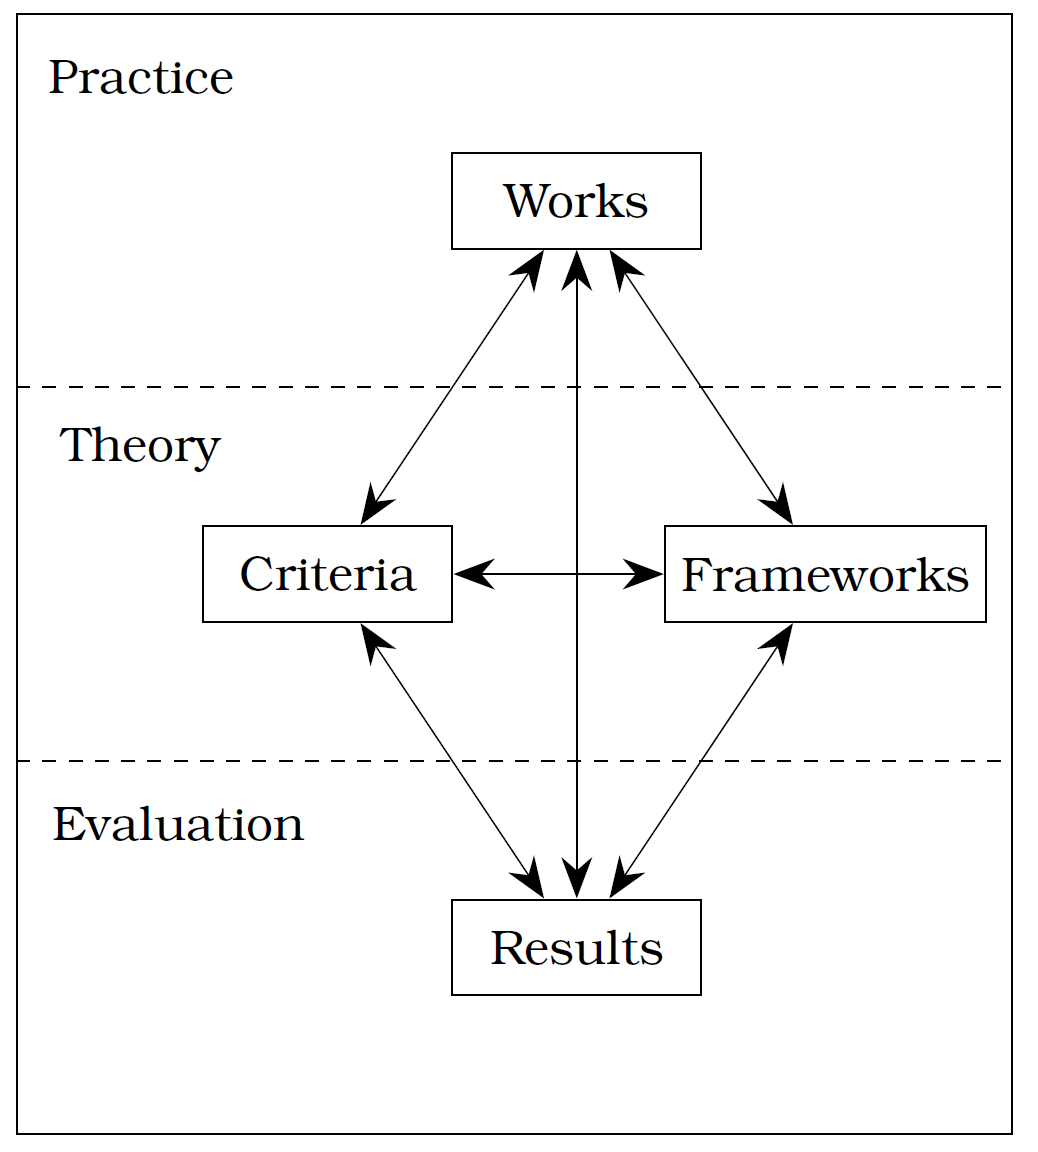
\includegraphics{images/tmpr}
  \caption[tmpr]{tmpr}
\label{fig:tmpr}
\end{figure}

``A framework comprises a conceptual structure that is used to influence practice, inform theory and, in particular, shape evaluation.''

``Some examples of framework types are:
• classifications for assessing the ways in which audiences respond to particular works.
• criteria for guiding the design of a new artifact or installation,
• questions, expressed as working hypotheses, to be explored using theoretical knowledge''

\begin{table}[htb]
  \begin{tabu}{X[1]X[2]X[3]}
  \toprule
  \textbf{Elements}
  &
  \textbf{Activities}
  &
  \textbf{Outcomes}
  \\ \midrule
  \textbf{Practice}
  &
  create, exhibit, reflect
  &
  \textbf{Works:} consisting of physical artefacts, musical compositions, software systems, installations, exhibitions, collaborations
  \\ \midrule
  \textbf{Theory}
  &
  read, think, write, develop
  &
  \textbf{Frameworks:} comprising questions, criteria, issues
  \\ \midrule
  \textbf{Evaluation}
  &
  observe, record, analyse, reflect
  &
  \textbf{Results:} findings leading to new/modified Works and Frameworks
  \\ \bottomrule
  \end{tabu}
\caption[Elements, Activities and Outcomes of the \gls{tmpr}]{Elements, Activities and Outcomes of each Trajectory in the \gls{tmpr}}
\label{tmprtable}
\end{table}

\begin{fcom}
  My project is using a practice based research methodology. A transdisciplinary epistemology. Method of constructing a prototype.
\end{fcom}



\section{Research Approach}



% NOTES

% \textbf{Information System}
% "An information system is not the information technology alone, but the system that emerges from the mutually transformational interactions between the information technology and the organization." \autocite{Mingers2004}
%
% \textbf{Inductive reasoning}
% "is a kind of reasoning that constructs or evaluates general propositions that are derived from specific examples. Inductive reasoning contrasts with deductive reasoning, in which specific examples are derived from general propositions." [wikipedia]
%
% \textbf{Specific to General}
% In an inductive approach you "collect data and develop theory as a result of your data analysis." \autocite{Knox2004}
%
% \textbf{Deductive reasoning}
% "is the process of reasoning from one or more general statements regarding what is known to reach a logically certain conclusion." [wikipedia]
%
% \textbf{General to Specific}
% In a deductive approach you "develop a theory and hypothesis (or hypotheses) and design a research strategy to test the hypothesis." \autocite{Knox2004}
%
% Positivism + quantitative methods + deduction
% vs
% Critical interpretivism + qualitative methods + induction
%
% \textbf{Positivism}
% "Positivism is a philosophy of science based on the view that in the social as well as natural sciences, data derived from sensory experience, and logical and mathematical treatments of such data, are together the exclusive source of all authoritative knowledge. Positivism assumes that there is valid knowledge (truth) only in scientific knowledge." [wikipedia]
%
% "Later antipositivists and critical theorists have associated positivism with "scientism"; science as ideology." [wikipedia]
%
% Heisenberg: "The positivists have a simple solution: the world must be divided into that which we can say clearly and the rest, which we had better pass over in silence. But can any one conceive of a more pointless philosophy, seeing that what we can say clearly amounts to next to nothing. If we omitted all that is unclear, we would probably be left with completely uninteresting and trivial tautologies." [wikipedia]
%
% Positivism is linked to deduction. \autocite{Knox2004}
%
% \textbf{Logical positivism}
% "(also known as logical empiricism, scientific philosophy, and neo-positivism)
% is a philosophy that combines empiricism—the idea that observational evidence is indispensable for knowledge—with a version of rationalism incorporating mathematical and logico-linguistic constructs and deductions of epistemology. It may be considered as a type of analytic philosophy." [wikipedia]
%
% \textbf{Interpretivism}
% "interpretivism (anti-positivism) may be equated with qualitative research methods, while positivist research is more quantitative. Positivists typically use research methods such as experiments and statistical surveys, while antipositivists use research methods which rely more on ethnographic fieldwork, conversation/discourse analysis or open-ended interviews. Positivist and antipositivist methods are sometimes combined." [wikipedia]
%
% Interpretivism is linked to induction. \autocite{Knox2004}
%
% \textbf{Functionalism}
% "functionalism emphazises the distinctness of, and the linkages among, individuals, culture or society." \autocite{Mingers2004}
%
% 1.	Functionalism is etic.
% 2.	Functionalist theory distinguishes between individuals and collectives.
% 3.	Functionalism holds that the parts of collectives are generally well integrated with each other, fulfilling the needs of the collectives and tending towards stability once equilibrium has been established. \autocite{Mingers2004}
%
% An 'emic' account is a description of behavior or a belief in terms meaningful (consciously or unconsciously) to the actor; that is, an emic account comes from a person within the culture. Almost anything from within a culture can provide an emic account. [wikipedia]
%
% An 'etic' account is a description of a behavior or belief by an observer, in terms that can be applied to other cultures; that is, an etic account attempts to be 'culturally neutral'. [wikipedia]
%
% [3]: \url{http://win.ua.ac.be/~sdemey/Tutorial_ResearchMethods/}
% 1.	Feasibility study (is it possible?)
% 2.	Pilot Case/Demonstrator (is it appropriate?)
% 3.	Comparative study (is it better?)
% 4.	Observational study (what is it?)
% 5.	Literature survey (what is known/unknown?)
% 6.	Formal Model (underlying concepts?)
% 7.	Simulation (what if?)
%
% \textbf{Phenomenology}
% "describes a body of knowledge that relates empirical observations of phenomena to each other, in a way that is consistent with fundamental theory, but is not directly derived from theory." [wikipedia]
%
% "A theory that expresses mathematically the results of observed phenomena without paying detailed attention to their fundamental significance." [Thewlis, J. (Ed.) (1973). Concise Dictionary of Physics. Oxford: Pergamon Press, p. 248.]
%
% "phenomenology is a transcendental approach to our understanding of the world." \autocite{Mingers2004}
%
% \textbf{Grounded theory}
% is a systematic methodology in the social sciences involving the discovery of theory through the analysis of data.\autocite{Mingers2004}[wikipedia] It is mainly used in qualitative research, but is also applicable to quantitative data. Grounded theory method is a research method which operates almost in a reverse fashion from traditional social science research. Rather than beginning with a hypothesis, the first step is data collection, through a variety of methods. From the data collected, the key points are marked with a series of codes, which are extracted from the text. The codes are grouped into similar concepts in order to make them more workable. From these concepts, categories are formed, which are the basis for the creation of a theory, or a reverse engineered hypothesis. This contradicts the traditional model of research, where the researcher chooses a theoretical framework, and only then applies this model to the phenomenon to be studied. [wikipedia]
%
% \textbf{Critical theory }
% is a school of thought that stresses the examination and the critique of society and culture. [wikipedia]
%
% \textbf{Philosophical and Methodological Pluralism}
% "Research is neatly divided into mutually exclusive categories, these being quantitative and qualitative research and ‘never the twain shall meet’. This divide is further strengthened with the inference that the relationship extends further; associating deduction with quantitative methods and similarly induction with qualitative methods." \autocite{Knox2004}
%
% "A method does not select a theory but […] there is an elective affinity between a theory and a method." \autocite{Knox2004}
%
% \textbf{Epistemological Pluralism}
% "Epistemologies … shape how researchers answer questions regarding the validity of knowledge (qualitative vs. quantitative, etc.), the legitimacy of methods to produce knowledge (experimentation, induction, hypothesis testing, etc.), and the assumptions inherent in particular conceptualizations of the object of study and certain methodologies." \autocite{Miller2008}
%
% \textbf{Evolving Methodology}
% "there can be no single prescribed methodology for TD research" \autocite{Wickson2006}
% Multidisciplinary research "tends to retain disciplinary autonomy" \autocite{Wickson2006}
% Interdisciplinary research "involves the development of a shared methodological approach across different disciplinary frameworks" \autocite{Wickson2006}
% Transdisciplinarity "is characterised by an interpenetration of epistemologies in the development of methodology" \autocite{Wickson2006} "the dissolution of disciplinary boundaries is necessary for the construction of novel or unique methodologies tailored to the problem and its context." \autocite{Wickson2006} "‘elements of methodologies drawn from different disciplines are combined within a single approach … an evolved methodology" \autocite{Wickson2006} "Transdisciplinarity arises only if research is based upon a common theoretical understanding and must be accompanied by a mutual interpenetration of disciplinary epistemologies" \autocite{Wickson2006}
%
% ``Characterising TD research by the process of having multiple research approaches critiquing and deconstructing one another to develop an evolved methodology resonates with Ramadier’s concept of ‘‘collaborative deconstruction’’.'' \autocite{Wickson2006}
%
% ``The foregrounding of collaboration as a distinguishing feature of transdisciplinarity raises the question as to whether it is possible for a lone researcher to undertake TD research. Emphasising the importance of collaboration for TD research would seem to imply that the research requires a group of individuals from a range of different disciplines to come together to conduct research, precluding individuals from researching in a TD manner. If however, we see the distinguishing feature of transdisciplinarity as not simply collaboration between researchers from different disciplines, but as collaboration with the community, then this allows the possibility for lone researchers to adopt TD approaches. What becomes important then is the ability of the individual to fuse knowledge from a number of different disciplines and engage with stakeholders in the process of generating knowledge. Individuals undertaking TD research could be discipline-based researchers who have simply chosen to adopt TD approaches for a particular project, or they could be researchers who have specifically adopted TD approaches as their primary modus operandi. We contend that having researchers who regularly operate in a TD manner would foster the development of the unique integrative and collaborative skills required in TD research. These TD researchers would then have the potential to act as catalysts, instigating and facilitating TD research across a range of disciplinary and institutional contexts and building bridges between disciplines, researchers and communities.'' \autocite{Wickson2006}
%
% ``On one level, TD researchers are required to integrate knowledge from different disciplines.'' \autocite{Wickson2006}
%
% ``Julie Thompson Klein [16] draws attention to the way in which Nicolescu calls transdisciplinarity ‘‘the science and art of discovering ridges between different areas of knowledge and different beings’’.'' \autocite{Wickson2006}
%
% ``Praxis is defined in Fawcett, Bell and Russell [22] as the idea that theory and practice are related, in that theory should be grounded in practice and practice enriched by theory.'' \autocite{Wickson2006}
%
% ``This scale of integration suggests that the researcher develops a richer understanding of the problem if they are actually engaged with it… An inherent challenge associated with this dimension of integration is how to maintain some critical distance while working as an embedded researcher.'' \autocite{Wickson2006}
%
% ``This means that it becomes important for the researcher to reflect on how their own frames of reference/values/beliefs/assumptions etc have shaped the conceptualisation of the problem, as well as the development of the method of investigation and the solution.'' \autocite{Wickson2006}
%
% "One suggestion that has emerged in the theoretical literature is the notion of understanding paradoxes as relating to different levels of reality [20]." \autocite{Wickson2006}
%
% "For Henagulph [20],this notion of different levels of reality offers a way out of the binary logic that dominates modern Western thought and the problem of the paradox that it creates. Instead of an either/or approach to understanding the nature of reality, the idea of different levels of reality and the ‘‘logic of the included middle’’ enables us to conceptualise a way in which something can be both A and non-A." \autocite{Wickson2006}
%
"Thomas Mann has been quoted as suggesting that ‘‘A great truth is a truth whose opposite is also a great truth’’ [23]." \autocite{Wickson2006}
%
% \autocite{Wickson2006}
% •	How was the research problem formulated?
% •	What is the relationship between methodology and problem context?
% •	How have competing epistemologies been reconciled?
% •	How has collaboration featured in the project?
% •	How well have knots of communication between different bodies of knowledge been created? Is the weave informative, useful, compelling?
% •	Does the research acknowledge, resolve and/or accommodate paradox?
% •	How has the researcher reflected on, recognised or accounted for the limitations and subjectivities of their approach and project outcomes?
%
%
% \autocite{Wickson2006} : Glassick and others at the Carnegie Foundation [26].
% 1. Clear goals—the scholar identifies important questions in the field, clearly articulates the purpose of the work and defines realistic objectives.
% 2. Adequate preparation—the scholar demonstrates an understanding of existing knowl- edge in the field and brings the necessary skills and resources to the project.
% 3. Appropriate method—the scholar selects and effectively applies methods appropriate to the goals and modifies these methods in response to changing circumstances.
% 4. Significant results—the scholar achieves set goals, makes an important contribution to the field and highlights new areas for exploration.
% 5. Effective presentation—the scholar employs appropriate means (style, medium, forums etc) to clearly communicate the work to its intended audience.
% 6. Reflective critique—the scholar uses a breadth of evidence to critically evaluate their work and through this process improves the quality of future endeavours.
%
% \autocite{Wickson2006} Reformulated for TD:
% 1. Responsive goals—in TD research, the scholar defines goals through ongoing consultation with the problem context and stakeholders. Goals may therefore not be clear from the outset and may shift in response to developments over the course of the project.
% 2. Broad preparation—in TD research, ‘adequate preparation’ would require accessing and integrating literature and theory across a broad range of disciplines, as well as engaging with the problem in its broader context.
% 3. Evolving methodology—an ‘appropriate method’ for TD research is ideally epistemologically integrative and capable of evolving in response to a changing research context.
% 4. Significant outcome—the outcome of TD research should contribute to the solution of a manifest problem in a way that is capable of satisfying multiple agendas, for example, be concurrently socially robust, environmentally sustainable and economically viable.
% 5. Effective communication—in support of collaborative processes, TD research should initiate and maintain two way communication with stakeholders over the life of the project.
% 6. Communal reflection—in addition to personal reflection, TD research should include a more communal reflective process—multiple disciplinary and stakeholder perspectives informing and transforming each other throughout the life of the project.
%
%
% (Lawrence and Després, 2004)
% 1.	Transdisciplinarity tackles complexity in science and it challenges knowledge fragmentation [and is] characterised by its hybrid nature, non-linearity and reflexivity, transcending any academic disciplinary structure.
% 2.	Transdisciplinary research accepts local contexts and uncertainty; it is a context-specific negotiation of knowledge.
% 3.	Transdisciplinarity implies intercommunicative action. Transdisciplinary knowledge is the result of intersubjectivity. Transdisciplinary research and practice require close and continuous collaboration during all phases of a research project.
% 4.	Transdisciplinary research is often action-oriented.
%
% Nicolescu \autocite{Nicolescu2010}
% "All knowledge other than scientific knowledge is thus cast into the inferno of subjectivity, tolerated at most as a meaningless embellishment or rejected with contempt as a fantasy, an illusion, a regression, or a product of the imagination."
% \autocite{Nicolescu2010}
%
"Objectivity, set up as the supreme criterion of Truth, has one inevitable consequence: the transformation of the Subject into an Object. The death of the Subject is the price we pay for objective knowledge." \autocite{Nicolescu2010}
%
""The too strong insistence on the difference between scientific knowledge and artistic knowledge comes from the wrong idea that concepts describe perfectly the ‘real things.’ […] All true philosophy is situated on the threshold between science and poetry."" [Heisenberg as cited in 11]
%
% "Multidisciplinarity concerns itself with studying a research topic in not just one discipline but in several simultanously. From this perspective, any topic will ultimately be enriched by incorporating the perspectives of several disciplines. Multidisciplinarity brings a plus to the discipline in question, but this "plus" is always in the exclusive service of the home discipline. In other words, the multidisciplinary approach overflows disciplinary boundaries while its goal remains limited to the framework of disciplinary research.
%
% "Multidisciplinary research arises when multiple researchers investigate a single problem, but do so as if each were working within their own disciplinary setting." \autocite{Miller2008}
%
% Interdisciplinarity has a different goal than multidisciplinarity. It concerns the transfer of methods from one discipline to another. Like multidisciplinarity, interdisciplinarity overflows the disciplines, but its goal still remains within the framework of disciplinary research. Interdisciplinarity even has the capacity of generating new disciplines, such as quantum cosmology and chaos theory.
%
% "Interdisciplinary research incorporates a greater degree of integration than either disciplinary or multidisciplinary research. Unified problem formulation, sharing of methods, and perhaps the creation of new questions are aspects of this type of work. In addition, interdisciplinary work often has an applied orientation." \autocite{Miller2008}
%
% Transdisciplinarity concerns that which is at once between the disciplines, across the different disciplines, and beyond all disciplines. Its goal is the understanding of the present world, of which one of the imperatives is the unity of knowledge." \autocite{Nicolescu2010}
%
% "Transdisciplinary research transcends entrenched categories to formulate problems in new ways. Collaborators may accept an epistemological perspective unique to the effort, redrawing the boundaries between disciplinary knowledges. Transdisciplinary research is often, although not always, characterized by an explicit engagement with society." \autocite{Miller2008}
%
% "This simultaneous consideration of theoretical, phenomenological, and experimental transdisciplinarity will allow both a unified and non-dogmatic treatment of the transdisciplinary theory and practice, coexisting with a plurality of transdisciplinary models." \autocite{Nicolescu2010}
%
Three axioms of the methodology of transdisciplinarity:
1. The ontological axiom: There are, in Nature and society and in our knowledge of Nature and society, different levels of Reality of the Object and, correspondingly, different levels of Reality of the Subject.
2. The logical axiom: The passage from one level of Reality to another is ensured by the logic of the included middle.
3. The complexity axiom: The structure of the totality of levels of Reality or perception is a complex structure: every level is what it is because all the levels exist at the same time. \autocite{Nicolescu2010}
%
% "A new Principle of Relativity emerges from the coexistence between complex plurality and open unity in our approach: no level of Reality constitutes a privileged place from which one is able to understand all the other levels of Reality…. In other words, our approach is not hierarchical. … Every level is characterized by its incompleteness: the laws governing this level are just a part of the totality of laws governing all levels.'' \autocite{Nicolescu2010}
%
% ``the theorem of Kurt Gödel, which states that a sufficiently rich system of axioms inevitably leads to results that are either undecidable or contradictory. The implications of Gödel’s theorem have considerable importance for all modern theories of knowledge, primarily because it concerns not just the field of arithmetic but all of mathematics that include arithmetic. The Gödelian structure of levels of Reality implies the impossibility of a self-enclosed, complete theory. Knowledge is forever open.'' \autocite{Nicolescu2010}
%
% \textbf{The Excluded Middle}
% The three classic laws of thought are attributed to Aristotle and were foundational in scholastic logic. They are [wikipedia]:
% •	law of identity
% •	law of noncontradiction
% •	law of excluded middle
%
% \textbf{The Included Middle}
% ``The unity of levels of Reality and its complementary zone of non-resistance constitutes what we call the transdisciplinary Object. … The unity of levels of Reality of the Subject and this complementary zone of non-resistance consti- tutes what we call the transdisciplinary Subject. The two zones of non-resistance of transdisciplinary Object and Subject must be identical for the transdisciplinary Subject to communicate with the transdisciplinary Object. A flow of consciousness that coherently cuts across different levels of perception must correspond to the flow of information coher- ently cutting across different levels of Reality. The two flows are interrelated because they share the same zone of non-resistance…. The zone of non-resistance plays the role of a third between the Subject and the Object, an Interaction term, which acts like a secretly included middle that allows for the unification of the transdisciplinary Subject and the transdisciplinary Object while preserving their difference. I will call this Interaction term the Hidden Third.'' \autocite{Nicolescu2010}
%
``Our ternary partition (Subject, Object, Hidden Third) is, of course, different from the binary partition (Subject vs. Object) of classical realism.'' \autocite{Nicolescu2010}
%
% The classical logic is founded on three axioms: \autocite{Nicolescu2010}
% 1.	The axiom of identity: A is A.
% 2.	The axiom of non-contradiction: A is not non-A.
% 3.	The axiom of the excluded middle: There exists no third term T ("T" from "third") which is at the same time A and non-A.
%
% "The logic of the included middle does not abolish the logic of the excluded middle: it only constrains its sphere of validity." \autocite{Nicolescu2010}
%
% ``It is therefore useful to distinguish between the horizontal complexity, which refers to a single level of reality and vertical complexity, which refers to several levels of Reality. … From a transdisciplinary point of view, complexity is a modern form of the very ancient principle of universal interdependence.'' \autocite{Nicolescu2010}
%
% ``For transdisciplinarity, a Big Picture is not only possible but also vitally necessary, even if it will never be formulated as a closed theory.'' \autocite{Nicolescu2010}
%
``The old principle `unity in diversity and diversity from unity' is embodied in transdisciplinarity.'' \autocite{Nicolescu2010}
%
% CIRET - International Center for Transdisciplinary Research [12]
% ``Disciplinary research concerns, at most, one and the same level of Reality; moreover, in most cases, it only concerns fragments of one level of Reality. On the contrary, transdisciplinarity concerns the dynamics engendered by the action of several levels of Reality at once.''
%
``Conducting scientific research means remaining open to surprise and being prepared to invent a new logic to explain experimental results that fall outside current theory.'' \autocite{Jarry2006}
%
``Heisenberg’s Uncertainty Principle is merely an application, a demonstration of the Clinamen, subjective viewpoint and anthropocentrism all rolled into one.'' \autocite{Jarry2006}

\stopcontents[chapters]
